\documentclass[10pt]{article}
\usepackage{ctex}
\usepackage{graphicx}
\graphicspath{{E:/大学课程/大一下/人工智能程序设计/作业集/第十二周作业/图片集/},{pics/}}
\usepackage{amsmath}
\usepackage{amssymb}
\usepackage{float}%使图片紧跟在文字后面

\title{第九周问答作业}
\author{朱士杭\ 231300027}
\date{\kaishu \today}



\begin{document}
	\maketitle
	\section{问题一:广播如何逐元素加法}
	根据广播的原则,从后往前逐一匹配,对于数组A与数组B最后一个元素为5,得以匹配;然后再匹配倒数第2个元素,发现A是1,B是3,
	因此A的1应当广播成3;然后再比较倒数第三个元素这个时候数组B没有更高的axis因此会扩展一个axis并且与A进行相应的匹配成3,
	因此最后的数组形状为(3,3,5),将扩展之后的数组A与数组B再逐一进行加法操作。
	\section{问题二:广播数组乘法}
	在两个ndarray数组运算过程中,先会进行从右往左的匹配操作,当两个维度长度相等或者其中一个为1时,两者compatible,
	当其中一个矩阵维度不足时,用长度为1的新维度进行补充。而广播则是将长度为1的维度内容复制匹配另一矩阵对应长度
	对于维度为(2,1)数组A与维度为(1,3)数组B,从右往左匹配的时候发现都可以匹配的上,接下来进行广播,将A的1广播为3,
	B的1广播为2都形成(2,3)的数组,然后逐元素进行multiply操作,最终结果数组形状为(2,3)
	假设数组A为$[[a_{11}],[a_{21}]]$,数组B形状为$[[b11,b12,b13]]$,广播之后分别为$$[[a_{11},a_{11},a_{11}],[a_{21},a_{21},a_{21}]]$$
	$$[[b_{11},b_{12},b_{13}],[b_{11},b_{12},b_{13}]]$$则最终结果为
	\begin{equation}
		\begin{aligned}
				[[a_{11}*b_{11},a_{11}*b_{12},a_{11}*b_{13}],\\
			[a_{21}*b_{11},a_{21}*b_{12},a_{21}*b_{13}]]
		\end{aligned}
	\end{equation}
	\section{问题三:行主序与列主序}
	\begin{figure}[H]
		\centering
		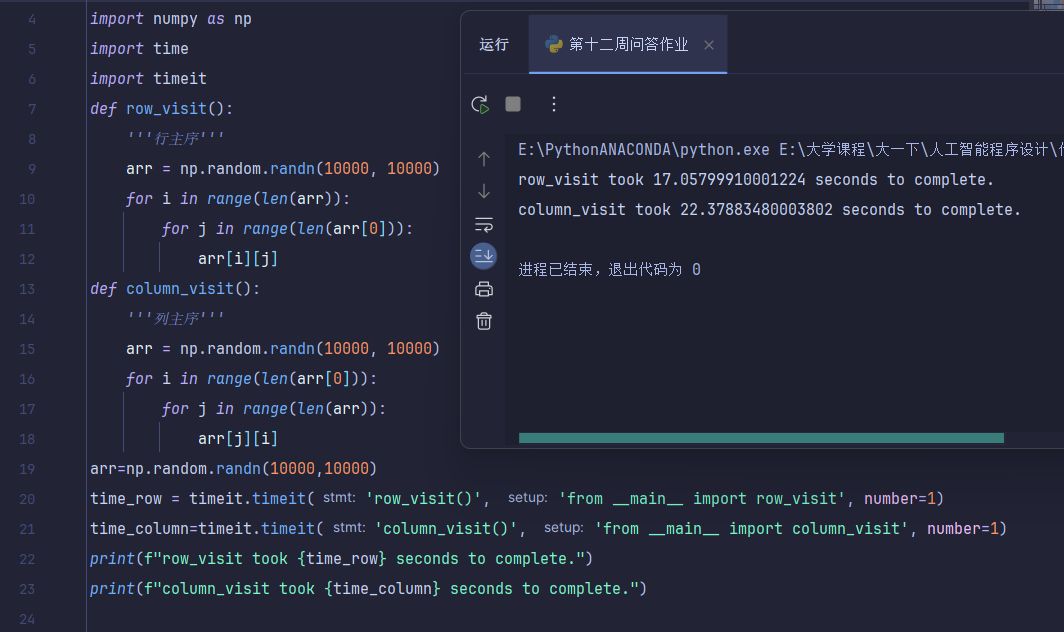
\includegraphics[scale=0.5]{优化前}
		\caption{行主序与列主序访问ndarray数组性能差异(优化前)}
	\end{figure}
	\begin{figure}[H]
		\centering
		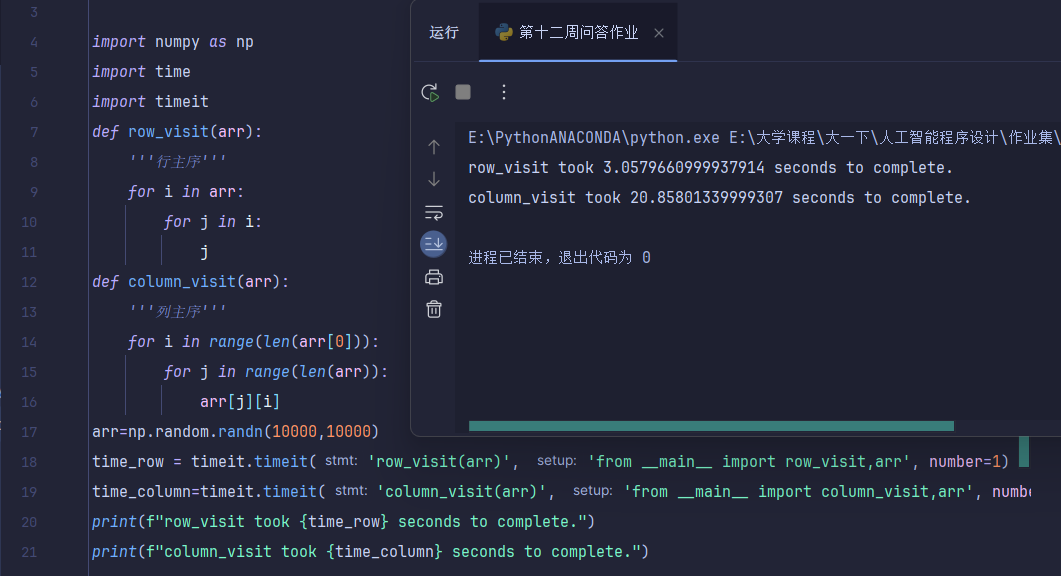
\includegraphics[scale=0.5]{优化后}
		\caption{行主序与列主序访问ndarray数组性能差异(优化后)}
	\end{figure}
	结果很明显,按行访问的时间效率远远高于按列访问的时间效率
	\subsection{为什么会有性能差异}在内部存储当中,numpy实际上是按照一行进行存储的,实际上就是一个一维数组,
	而计算机每一次从内存读取数据的时候都是先读一段到缓存当中(cpu当中的寄存机)\par
	由于时间重复性与空间重复性
	(即被访问的元素接下被再次访问到的概率更高,以及被访问的元素下面的元素被访问的概率也更高)因此同一行的元素被读进寄存器当中,
	如果按行进行访问的话每一次访问直接往下偏移即可,而如果按列进行访问的话,每一次又要从内存当中把下一行的数组读进寄存器当中,
	会大大降低时间效率
	
	
	\section{聚合函数}
	\subsection{聚合函数内部实现机制}
	NumPy的聚合函数有如np.mean、np.sum、np.max等,是NumPy中非常强大和常用的功能。
	这些函数可以沿着数组的指定轴进行操作,并且能够有效地处理多维数据。\par
	在内部实现上,这些NumPy聚合函数主要使用C语言编写,使得它能够高效地处理数组运算。
	当在多维数组上应用聚合函数时,NumPy会根据axis参数的值来确定如何遍历数组。
	axis参数指定了操作的轴,即沿着哪个维度进行聚合。
	NumPy内部存储当然是以一维数组去存储,并通过strides来确定访问某个元素的时候需要跳过多少个元素才能访问的到
	\subsection{如何指定axis参数}
	对于形状为(3,4,5)的三维数组,
	\subsubsection{如果按照axis=0进行聚合}
	确定strides为(20,5,1),
	然后根据0,1,2对3个(4,5)的块进行遍历累加求平均值(这里默认是跳过多少个元素而不是跳过多少个字节)
	最后变成一个(4,5)的二维数组
	\begin{figure}[H]
		\centering
		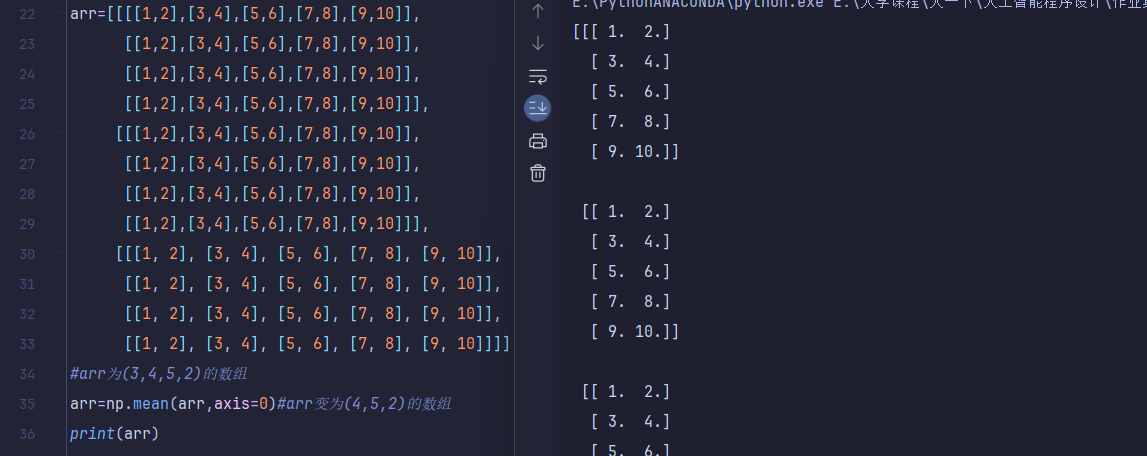
\includegraphics[scale=0.5]{mean}
		\caption{使用mean函数将一个(3,4,5,2)的数组按照axis=0进行聚合}
	\end{figure}
	\subsubsection{如果按照axis=1进行聚合}
	如果要按照axis=1进行聚合,对4个(3,5)的块进行遍历累加
	\subsubsection{如果按照axis=0进行聚合}
	如果要按照axis=2进行聚合,对5个(3,4)的块进行遍历累加
	\subsection{背后的数据迭代逻辑}
	在内部,NumPy使用了一种strider步进器来遍历数组。
	步进器是一种包含数组元数据和如何遍历数组的信息的数据结构,
	当一个聚合函数被调用时,NumPy会创建一个步进器来遍历数组,
	对于每个轴,步进器会计算该轴的步长strides跳过多少个元素到达下一个沿着该轴的元素,
	在多维数组中,步进器会根据axis参数来确定如何遍历数组
	
	
	\section{聚合函数的具体应用}
	\begin{figure}[H]
		\centering
		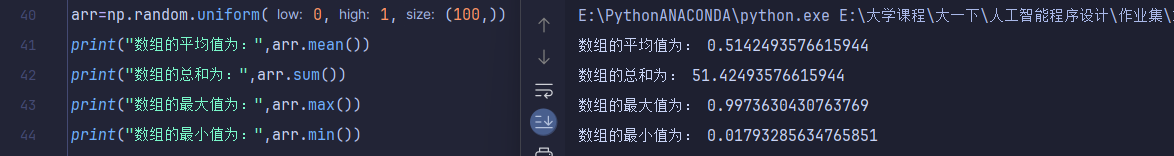
\includegraphics[scale=0.5]{100}
		\caption{计算并打印ndarray数组平均值、总和、最大值和最小值}
	\end{figure}
	
	\section{条件函数筛选ndarray数组}
		\begin{figure}[H]
		\centering
		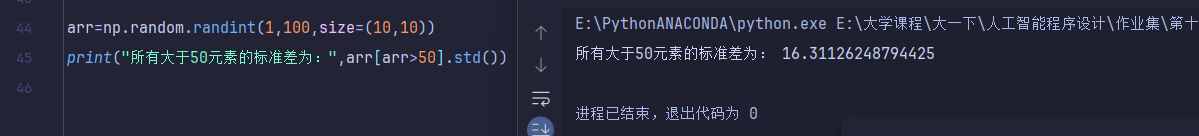
\includegraphics[scale=0.5]{1010}
		\caption{条件函数筛选大于50元素,并计算这些元素标准差}
	\end{figure}
	
	\section{三维矩阵类ThreeDimMatrix}
	\begin{figure}[H]
		\centering
		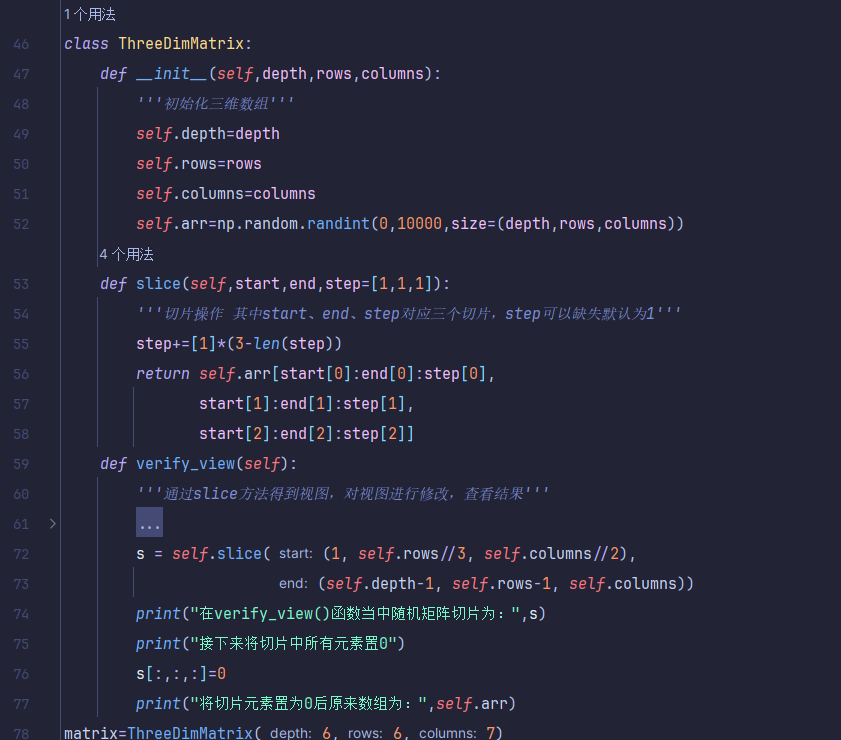
\includegraphics[scale=0.5]{类}
		\caption{定义一个三维矩阵类ThreeDimMatrix}
	\end{figure}
	首先先定义一个三维矩阵类ThreeDimMatrix,其中包含初始化、切片操作、视图验证三个成员函数
	\begin{figure}[H]
		\centering
		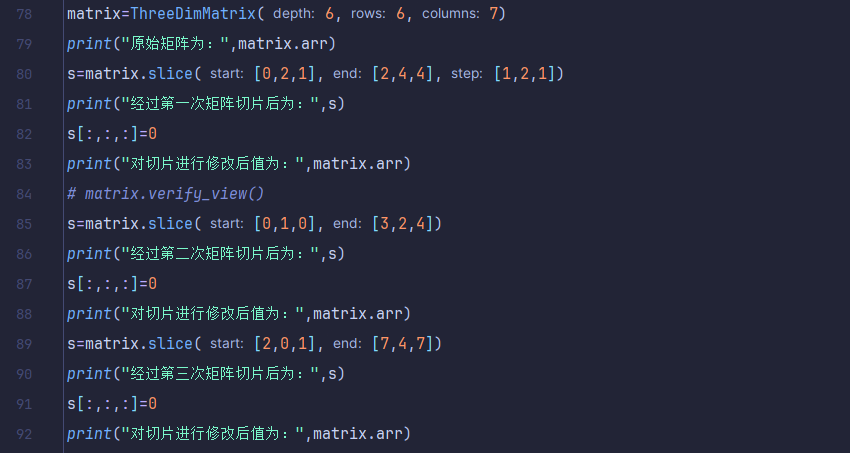
\includegraphics[scale=0.42]{切片}
		\caption{多次切片操作}
	\end{figure}
	然后实例化之后再进行多次切片操作,并且将视图值全部置为0,并且查看最终的修改结果
	\begin{figure}[H]
		\centering
		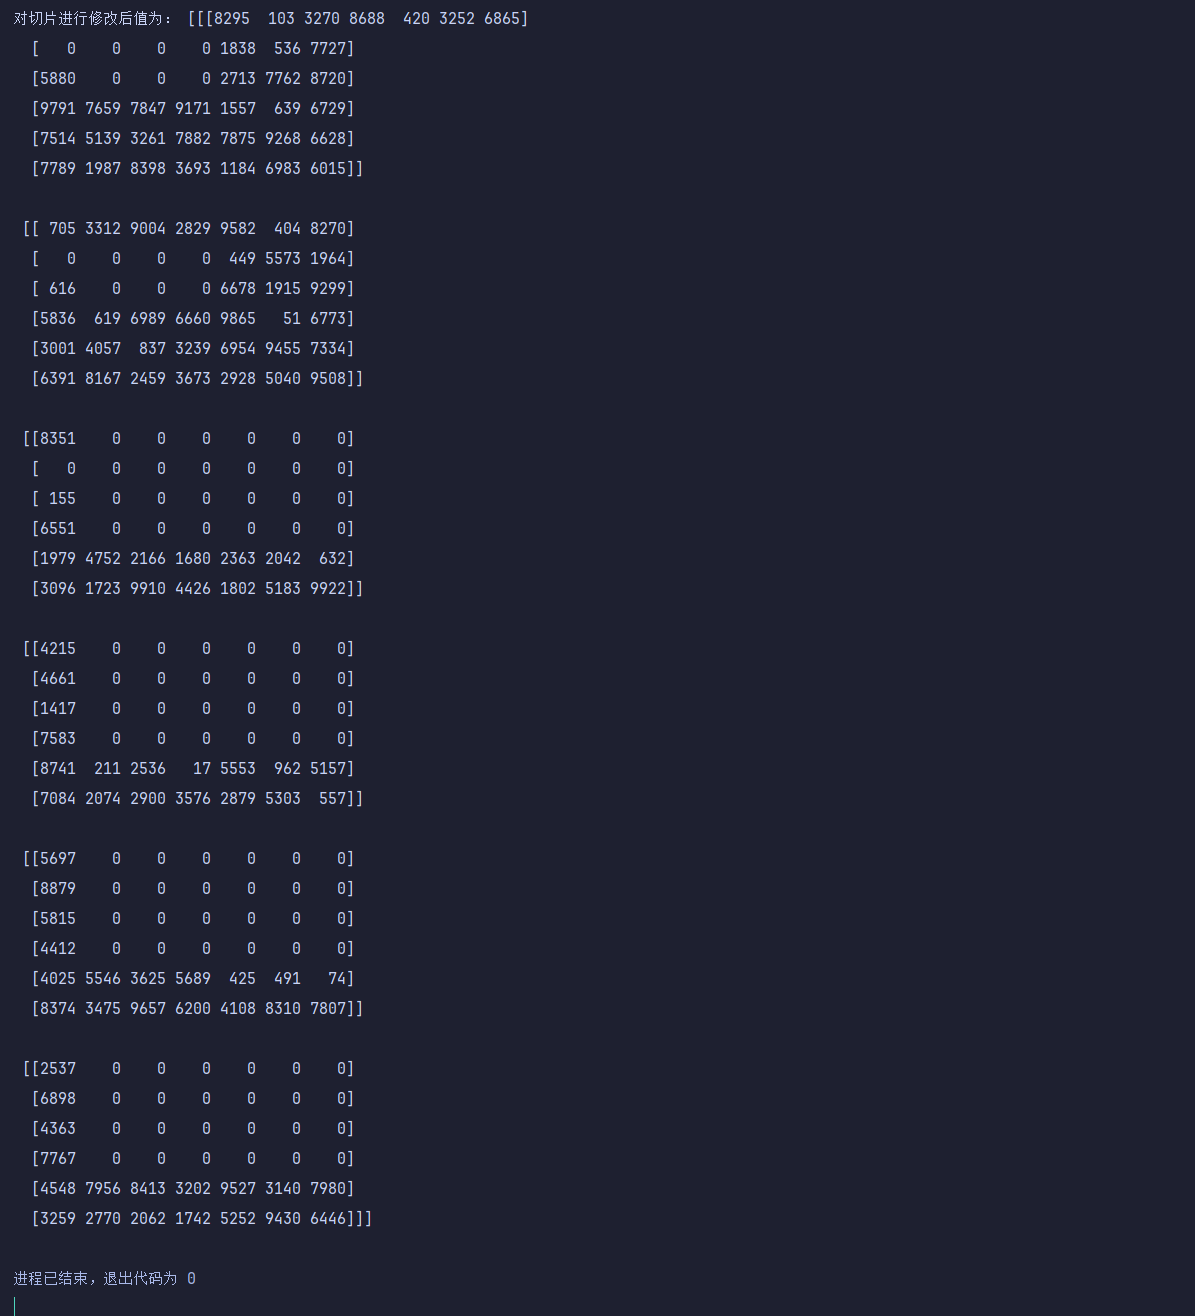
\includegraphics[scale=0.34]{结果}
		\caption{对视图的修改影响原始矩阵}
	\end{figure}
	最后发现对于视图的修改是会影响到原始矩阵的,因此可以得出结论,视图并不会创建新的ndarray数组对象,而是在原先的数组当中直接进行修改
\end{document}




